\begin{center}
    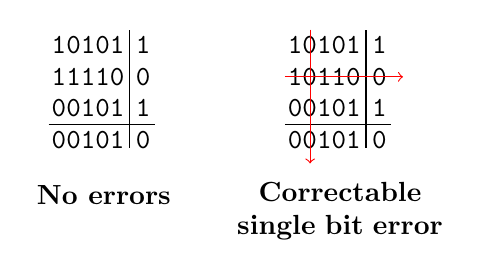
\begin{tikzpicture}
        %%%%%%%% Testo 1 %%%%%%%%%
        \node at (0,0) {\texttt{00101}};
        \node at (0,0.4) {\texttt{00101}};
        \node at (0,0.8) {\texttt{11110}};
        \node at (0,1.2) {\texttt{10101}};
        \node at (0.7,0) {\texttt{0}};
        \node at (0.7,0.4) {\texttt{1}};
        \node at (0.7,0.8) {\texttt{0}};
        \node at (0.7,1.2) {\texttt{1}};

        %%%%%%%% Schema 1 %%%%%%%%
        \draw (0.53,-0.1) -- (0.53,1.4);
        \draw (-0.5,0.2) -- (0.85,0.2);

        %%%%%%%% Testo 2 %%%%%%%%%
        \node at (3,0) {\texttt{00101}};
        \node at (3,0.4) {\texttt{00101}};
        \node at (3,0.8) {\texttt{10110}};
        \node at (3,1.2) {\texttt{10101}};
        \node at (3.7,0) {\texttt{0}};
        \node at (3.7,0.4) {\texttt{1}};
        \node at (3.7,0.8) {\texttt{0}};
        \node at (3.7,1.2) {\texttt{1}};

        %%%%%%%% Schema 2 %%%%%%%%
        \draw (3.53,-0.1) -- (3.53,1.4);
        \draw (2.5,0.2) -- (3.85,0.2);
        \draw[->,red] (2.5,0.8) -- (4,0.8);
        \draw[->,red] (2.82,1.4) -- (2.82,-0.3);

        %%%%%%%% Captions %%%%%%%%
        \node at (0.2,-0.7) {\textbf{No errors}};
        \node[text width=2.7cm,align=center] at (3.2,-0.9) {\textbf{Correctable single bit error}};
    \end{tikzpicture}
\end{center}